\newcommand{\CLASSINPUTtoptextmargin}{2cm}
\newcommand{\CLASSINPUTbottomtextmargin}{2cm}
\documentclass[journal,10pt,a4paper]{IEEEtran}
\usepackage{graphicx}
\usepackage{chngpage}
\usepackage{amsmath}
\usepackage{multirow}
\newcommand{\subparagraph}{}
% \usepackage [english]{babel}
% \usepackage [autostyle, english = american]{csquotes}
\usepackage{pgfplots}
\usepackage{pgfplotstable}
\usepackage{mathtools}
\usepackage{multicol}
\usepackage{titlesec}
\usepackage{gensymb}
\usepackage[justification=centering]{caption}
\usepackage{amsmath}
\usepackage{algorithm}
\usepackage[noend]{algpseudocode}
\usepackage{url}
\usepackage[final]{pdfpages}
%\usepackage{appendix}
\usepackage{float}
\usepackage{listings}
\usepackage{subfig}
 \usepackage[
    backend=biber,
    style=ieee,
  ]{biblatex}
\addbibresource{main.bib}
\setlength{\parskip}{0.5
em}

\renewcommand{\baselinestretch}{1.5}


\definecolor{mygreen}{rgb}{0,0.6,0}
\definecolor{mygray}{rgb}{0.5,0.5,0.5}
\definecolor{mymauve}{rgb}{0.58,0,0.82}


\lstset{language=python,
breaklines=true,
commentstyle=\color{mygreen},
 keywordstyle=\color{blue},
 stringstyle=\color{mymauve},
 morecomment=[l]{//}}







% *** GRAPHICS RELATED PACKAGES ***
%
\ifCLASSINFOpdf
  % \usepackage[pdftex]{graphicx}
  % declare the path(s) where your graphic files are
  % \graphicspath{{../pdf/}{../jpeg/}}
  % and their extensions so you won't have to specify these with
  % every instance of \includegraphics
  % \DeclareGraphicsExtensions{.pdf,.jpeg,.png}
\else
  % or other class option (dvipsone, dvipdf, if not using dvips). graphicx
  % will default to the driver specified in the system graphics.cfg if no
  % driver is specified.
  % \usepackage[dvips]{graphicx}
  % declare the path(s) where your graphic files are
  % \graphicspath{{../eps/}}
  % and their extensions so you won't have to specify these with
  % every instance of \includegraphics
  % \DeclareGraphicsExtensions{.eps}
\fi

% correct bad hyphenation here
\hyphenation{op-tical net-works semi-conduc-tor}

\graphicspath{{imgs/}{}}
\begin{document}
%
% paper title
% Titles are generally capitalized except for words such as a, an, and, as,
% at, but, by, for, in, nor, of, on, or, the, to and up, which are usually
% not capitalized unless they are the first or last word of the title.
% Linebreaks \\ can be used within to get better formatting as desired.
% Do not put math or special symbols in the title.
\title{A Comparison of MPI Two-Sided and One-Sided Communication Performance}

\author{Junaid Dawood (1094837), Xongile Nghatsane (1110680), Marissa van Wyngaardt (719804)}% <-this % stops a space



\maketitle

% As a general rule, do not put math, special symbols or citations
% in the abstract or keywords.

\begin{abstract}
This report presents a performance comparison of MPI's two-sided and one-sided approaches to inter-process communication. This performance comparison is made with reference to implementations of a parallel block-based matrix transposition algorithm which scales with the number of processes used. Results from the testing conducted suggest that the two-sided approach offers superior performance for sufficiently large matrices. In addition, it is found that the use of a collective I/O based scheme is a viable alternative to the two main strategies presented within this report, regardless of the communication method used.

\end{abstract}

\IEEEpeerreviewmaketitle

\section{Introduction}
Message Passing Interface (MPI) is a message passing standard which is designed to function on a diverse range of parallel computing architectures \cite{MPIAMess20:online}. Message passing typically achieves parallelism through messages passed between processes in order to transfer data. Popular implementations of the MPI standard for message passing include OpenMPI and MPICH \cite{ompi,mpich}.

MPI typically facilitates the use of the `single-program-multiple-data' (SPMD) parallelism model; as all nodes essentially run the same program. However, this is not required as many MPI implementations allow for multiple executables to exist within one MPI job. 

This report presents a performance comparison of two MPI-based implementations of block-based matrix transposition \cite{transp}, parallelised amongst many processes. These implementations differ in the type of communication used: the first makes use of MPI's typical two-sided communication, using \textit{Send} and \textit{Recv}. The second implementation uses MPI's one-sided communication \cite{one}, making use of \textit{Windows} and \textit{Get}.

\section{Background}

MPI's communication model is typically point-to-point in nature. That is, inter-process communication wherein both the receiver and sender are specified. That said, MPI also allows for \textit{broadcast} and \textit{receive-from-any} communication. MPI communication is typically two-sided i.e. it consists of distinct send and receive stages. For every send there must be an associated receive (if data is to actually reach its destination). Depending on the MPI implementation, a process may need its sent message to be acknowledged by a receiver, through a \textit{Recv} call, before it can continue with the rest of its processing.

In addition, MPI does allow for one-sided communication, which was included in the MPI-2 standard \cite{one,one1}. One-sided communication removes the necessity for the acknowledgement that exists within the conventional two-sided approach. Essentially, one-sided communication consists of making a \textit{Window} of a process' address space accessible to other processes; with the host process facilitating the opening and closing of the \textit{Window}. Other processes can then write or read from the \textit{Window}, as long as it remains open. This removes the need for the host process to wait for acknowledgements from those processes which require data that it holds.


\subsection{Problem Description and Success Criteria}

The brief problem statement included in the introduction must be expanded so as to fully describe the nature of this research. The matrix transposition implementation is intended to work on large data sets; which are to be stored, out-of-core, in external files. Note: matrices are stored in row major order within binary files for all implementations; individual matrix items are of the \textit{short} datatype.

The transposition implementations must be parallelised using the two MPI approaches mentioned earlier i.e. both one-sided and two-sided communication.

As described in the introduction, the algorithms discussed in this report pertain specifically to `block-based' transposition algorithms. This essentially entails splitting a large matrix into equally sized submatrices, transposing these submatrices, and performing the appropriate submatrix swaps.

Assuming there is a $N\times N$ matrix $A$ which can be written in terms of its $K \times K$ submatrices:

\begin{equation}
A=
\begin{bmatrix}
    W       & X \\
   Y&Z \\
\end{bmatrix}
\end{equation}


it can be proved that:
\begin{equation}
    A^T=
\begin{bmatrix}
    W^T       & Y^T \\
   X^T&Z^T \\
\end{bmatrix}
\end{equation}



This can be generalised to any square matrix which can be split into submatrices of equal size. However, this research focuses on square matrices of dimension $2^x$ by $2^x$, where $x$ is an integer satisfying $x\geq 3$. The block-based approach is limited to a minimum submatrix dimension of $2\times 2$, as there is no smaller meaningful block size. That said, it is likely that splitting input matrices into such small submatrices will involve larger communication overhead; leading to lower performance. However, this is more formally discussed later in this report.




\section{Conventional Implementation}

This implementation of the block-based transposition can be discussed in 4 stages: 1) Generation of matrix data, 2) Performing per-process transpositions, 3) Transmission of data to the master node, and 4) Writing of results to a file by the master node. Essentially, each process generates its own submatrix, transposes it, and passes the transposed matrix to the master process, which subsequently writes the entire transposed matrix to a file.

%Note that the differences between the one-sided and two-sided communication approaches only manifests within the thrid stage of the implementation.


\subsection{Generating Matrix Data}

Matrix data is generated on a per-process basis, through typical random number generation techniques. Each process generates its own, equally sized, submatrix. The size of the submatrices is determined by the desired size of the overall matrix which is being transposed. If the number of available processes is so large that an even distribution would yield submatrices smaller than $2 \times 2$, then some processes are left out of the transposition entirely, in order to impose the $2 \times 2$ minimum submatrix size. Similarly, processes are sometimes excluded to ensure that each process only ever performs a transposition on a single square submatrix.

%The reading operations used within this implementation are MPI's collective I/O functions, specifically the \textit{MPI File read all} function. Each process defines its own file view based on a common \textit{filetype}, as described below, and different offset value. In doing so, each process is able to appropriately read the data for its associated submatrix despite reads being done collectively. 


\subsection{Performing Submatrix Transpositions}

Each process, upon completing its submatrix generation, then performs a transposition on said submatrix. This submatrix transposition is done using a naive approach, which is parallelised using OpenMP \cite{omp}. The naive approach entails the typical per-element row-to-column coordinate transformation swaps.

\subsection{Data Transmission}

Within this two-sided communication approach, all participating processes will send their submatrices to the master node (rank 0) upon completing their respective transpositions. This is done through typical \textit{Send} and \textit{Recv} semantics. Essentially, the master node will receive each submatrix as a contiguous buffer, storing all of the received submatrices within a single, larger, contiguous buffer which is held locally.

\subsection{Writing of Transposed Matrix to File}

The master node is responsible for writing the transposed matrix to an output file. This is implemented using the \textit{File-writ}e and \textit{File-write-at} functions. The master node performs the necessary calculations for transforming its continuous buffer representation of the matrix to the final row-major ordered contents of the output file. This involves calculating write offsets for each submatrix and writing these submatrices at the locations specified by said offsets. Each row of each submatrix is written consecutively; applying an offset equivalent to the size of the original matrix ($N$), after writing each row.



\section{One-Sided Approach}

The implementation of the one-sided approach is largely the same as the conventional \textit{Send} and \textit{Recv} implementation. The one-sided implementation differs only in the way in which data is exchanged between processes and the way in which data is written to the output file.

\subsection{Generating Matrix Data}
Like the two-sided approach, submatrices are generated on a per-process basis. As before, processes are sometimes excluded to maintain a minimum block size of $2 \times 2$, or to maintain square submatrices.


\subsection{Performing Submatrix Transpositions}
For fairness, the one-sided approach does not attempt to improve on the parallelised naive approach used in the two-sided implementation.

\subsection{Data Transmission}
This implementation makes use of MPI's one-sided communications for data transmission. All participating processes open a \textit{Window}; placing their local submatrix buffers within their respective \textit{Windows}. The master node then performs \textit{Get} operations on the contents of all these windows, such that it acquires all of the transposed submatrices required to construct the overall transposed matrix. The submatrices obtained through the \textit{Get} operations are stored within a single contiguous buffer on the master node.


\subsection{Writing of Transposed Matrix to File}

Like before, the master node is responsible for writing the contents of a contiguous buffer to an output file. However, this approach makes use of an MPI derived type in order to do so. Specifically, the MPI \textit{Vector} derived type is used to set a \textit{file view} for the writing of each submatrix to the output file. The stride length used for this derived data type is equal to the row length of the overall matrix $N$, the block length is equal to the row length of the submatrices $k$, and the count is equal to $N \times k$, as shown in figure \ref{fig:stride}. Constructing the file view in this way allows each submatrix to be written to the file within a single write call; unlike the I/O strategy used in the two-sided approach. 


\begin{figure}[H]
    \centering
    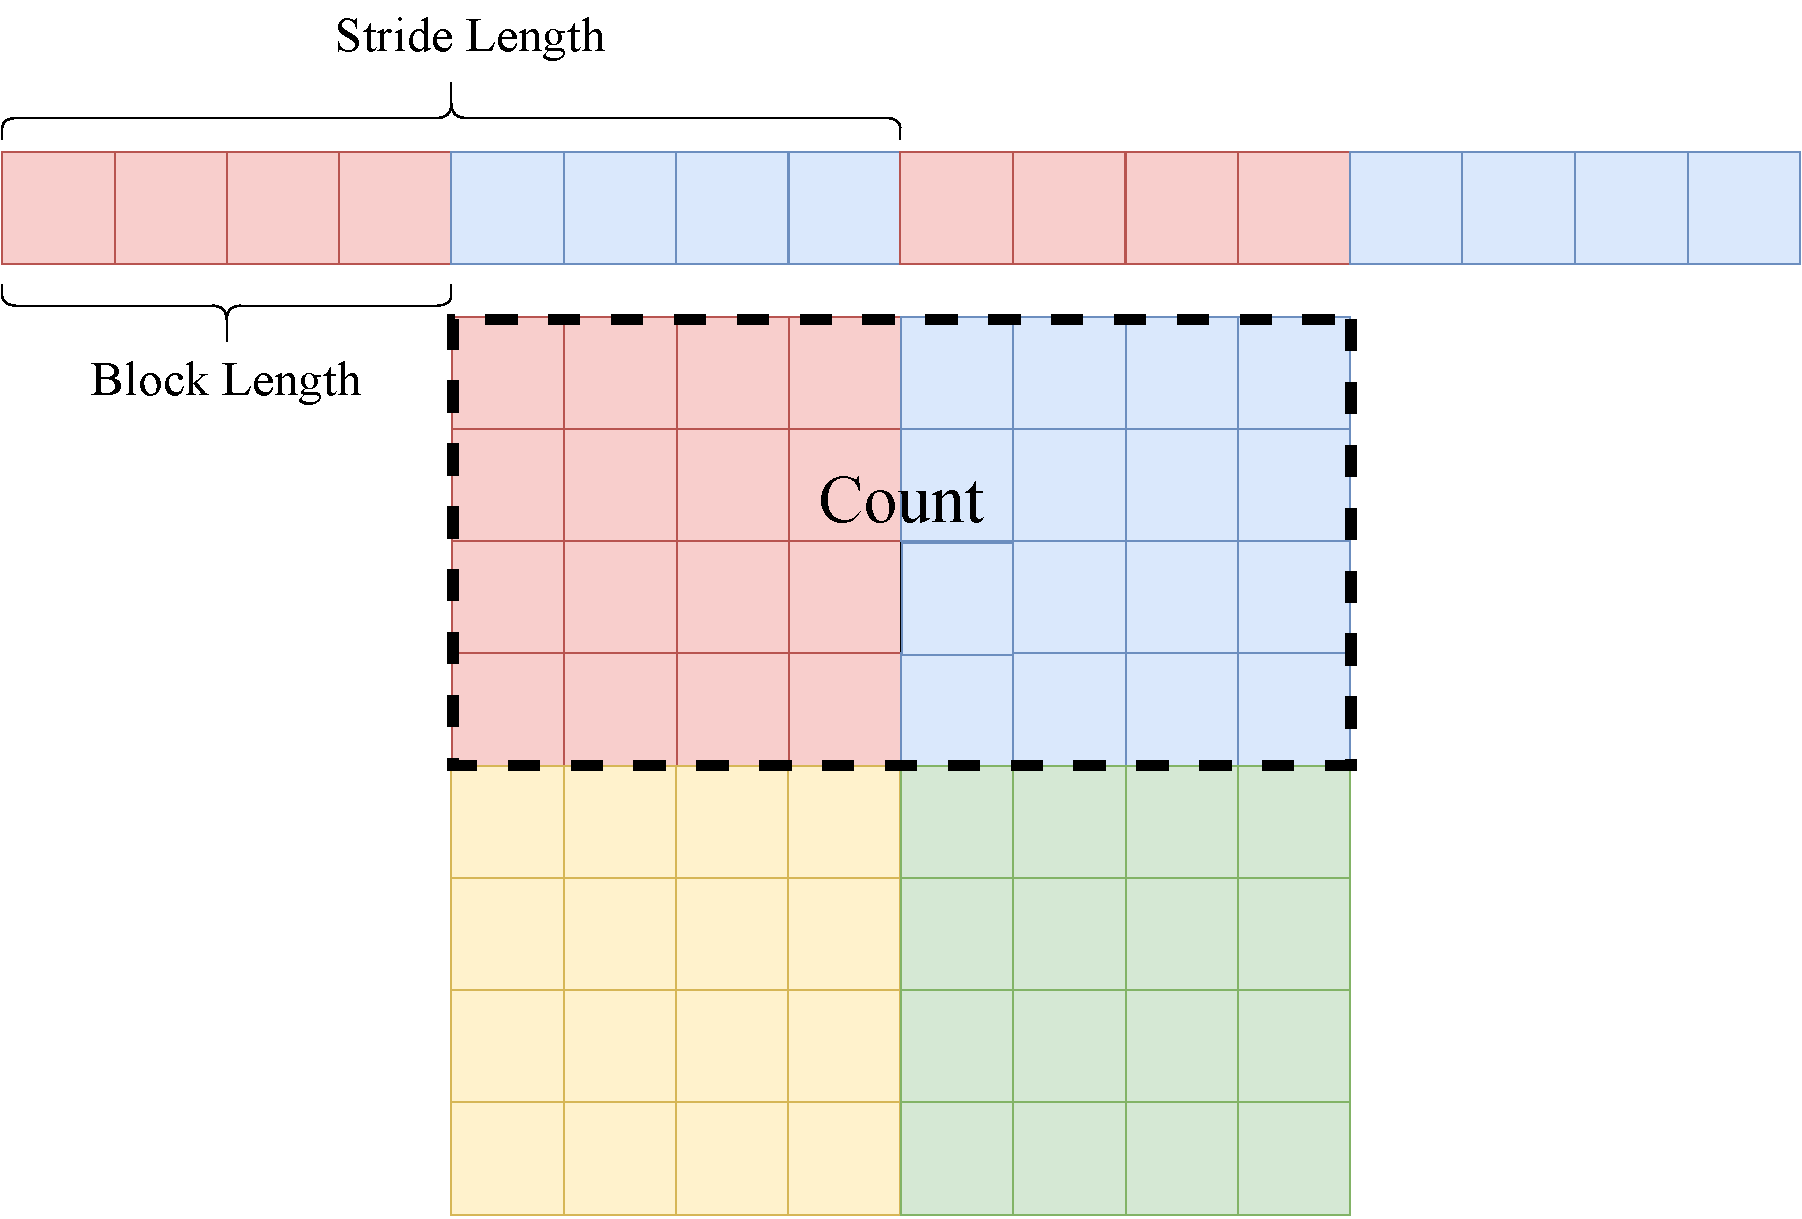
\includegraphics[width=0.35\textwidth]{stride.pdf}
    \caption{Derived type file view mapping.}
    \label{fig:stride}
\end{figure}

% \section{PGAS (UPC) Implementation}
% The UPC implementation is almost entirely the same as the MPI implementation discussed earlier. The only difference is the way in which inter-process data sharing is implemented. That is, the writing and reading of transposed matrices to a global array as opposed to fetching the matrices directly, from corresponding processes.

% \subsection{Reading Input Data}
% The reading of input data is implemented in manner which is almost identical to the MPI approach. All of UPC's I/O read/write functions are collective; thus an accurate comparison can be made between the UPC implementation and the MPI implementation.

% Achieving non-contiguous file reading in BUPC, using its LIST I/O functions, is far more complex than the use of file views and offets. Indeed, the process is more manual in nature, to the extent that no real simplification is offered. Thus, within this implementation \textit{strided} reading and writing of files is implemented manually using typical BUPC collective I/O functions as opposed to the LIST I/O functionality present.

% \subsection{Submatrix Transpositions}
% The transposition of submatrices in the UPC implementation is implemented in exactly the same way as the submatrix transposition of the MPI implementation, i.e. a naive approach. This is done so as to ensure no bias in performance comparisons.

% \subsection{Writing to the Shared Array}
% After transposing their respective submatrices, processes will write the contents of said submatrices in row-major order. The write locations are based on the intended output locations of the submatrix i.e. the write locations incorporate the block swapping step implicitly. That is, the offset used in this write step is equivalent to the offset used by the corresponding process in the reading-in phase.

% \subsection{Writing Output Data}

% Again, the writing of output data is almost identical to the MPI implementation, with the exception of the use of an explicit \textit{seek} method as described earlier. Data is copied directly from the shared array to the file using the \textit{upc all fwrite shared} function. That is, there is no need to copy the shared data to a local buffer before writing said data to a file.

% \subsection{Limitations}
% As is the case for the MPI implementation, submatrices must be at least $2x2$ in size. 





\section{Alternative Collective I/O Implementations}

Two alternative approaches are implemented to demonstrate the use of collective I/O in MPI \cite{io,io2} i.e. \textit{Read all} and \textit{Write all}. It is thought that these implementations will be able to highlight the bottleneck which occurs when a single node is responsible for performing I/O. These two alternatives differ in that one makes use of one-sided communication and the other, two-sided. This is done to afford fair, independent, comparisons of the use of collective I/O with the implementations discussed earlier.

\subsection{Input Data Generation}

Both of the collective I/O alternatives source their matrix data from an external file. This file is read from using a non-contiguous \textit{file view}: these \textit{file views} are consistent across all involved processes, except for the offsets used. The involved processes make use of a single collective \textit{Read all} call to populate their local submatrix buffers with values read from the file. 

%This is very similar the approach used for the writing of output data for the original one-sided communication approach.


\subsection{Submatrix Transposition}
Submatrix transposition remains unchanged from the parallelised naive approach discussed earlier. This ensures fairness of comparison between the alternatives and the two original approaches.

\subsection{Data Transmission}

Since the goal of these alternatives is the use of collective I/O, neither of the two alternatives require the sending of data to a master node for I/O purposes. Thus, processes need only swap their transposed submatrices, with those of corresponding processes. The mapping of these swaps is described by the diagram shown below: there is essentially a block-level transposition which occurs in this process.


\begin{figure}[H]
    \centering
    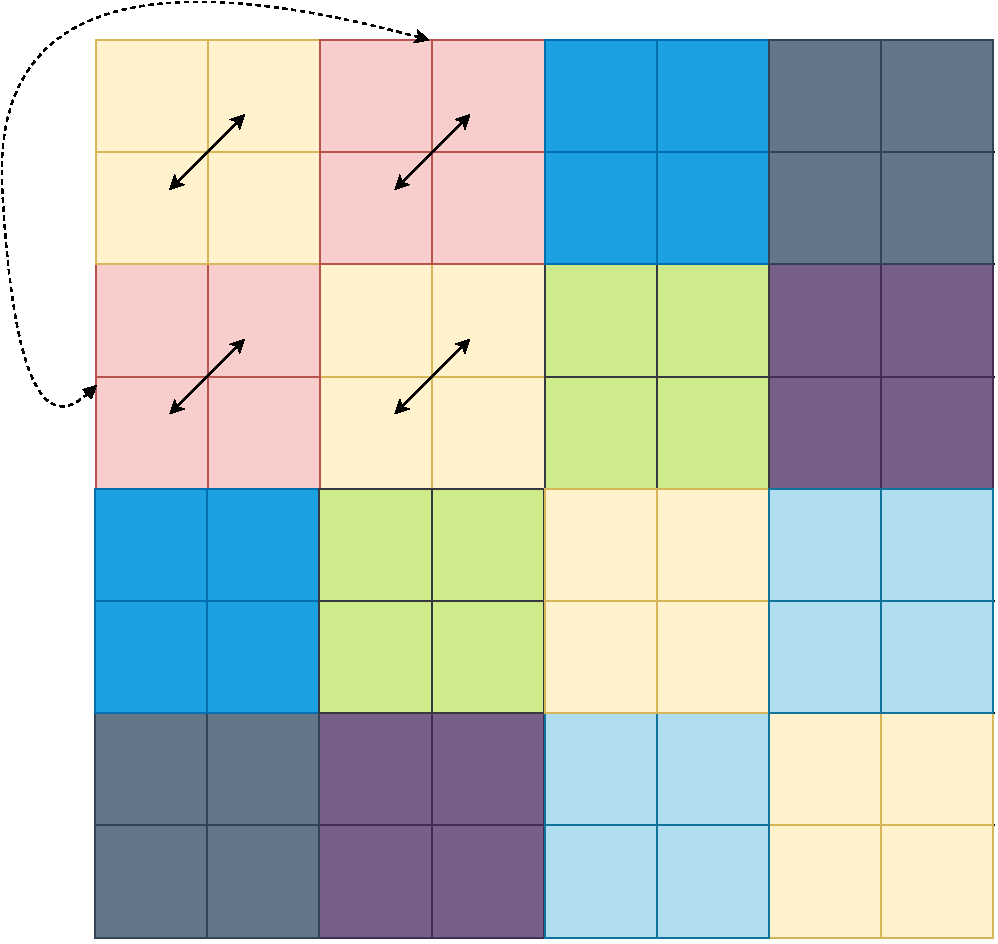
\includegraphics[width=0.3\textwidth]{block.pdf}
    \caption{Mapping of inter-process block swapping.}
    \label{fig:my_label}
\end{figure}

Of course, one of the alternatives does this through typical MPI \textit{Send} and \textit{Recv} commands whilst the other makes use of \textit{Windows} and \textit{Get} operations.


% That said, this is no different to the two approache

\subsection{Writing Output Data}

This step is very similar to the initial input data reading step. Once a process has obtained its corresponding block data, it is able to write this block to the output file. This is done through the use of a derived data type (\textit{Vector}) used to create a \textit{file view} such that each process can write its entire submatrix to a file within a single collective \textit{Write all} call.% Again, MPI's collective I/O is used in the form of the \texit{MPI File write all} function.

It should be noted that the offsets and filetype used to define file views used when writing to the output file are the same as those used when reading data from the input file, for any given process. The following two diagrams contrast the nature of the collective I/O approaches and the two approaches discussed earlier.

\begin{figure}[H]
    \centering
    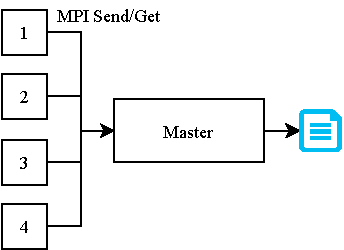
\includegraphics[width=0.3\textwidth]{norm.pdf}
    \caption{General structure of two main approaches.}
    \label{fig:my_label}
\end{figure}

\begin{figure}[H]
    \centering
    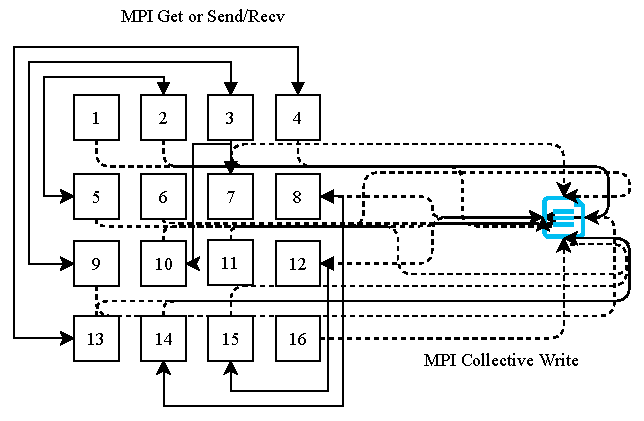
\includegraphics[width=0.45\textwidth]{col.pdf}
    \caption{General structure of two collective approaches.}
    \label{fig:my_label}
\end{figure}



\subsection{Limitations}
Since both of these approaches rely, inflexibly, on evenly distributing blocks amongst threads, they are incapable of catering to scenarios in which the number of available processes is greater than the number of $2\times 2$ blocks which can be yielded from the input matrix.








\section{Testing Environment and Procedure}

The implementations were sequentially tested on a cluster with NFS support. The number of processes used included 16, 32, and 64. Input matrices ranged in size from $8\times 8$ to $128\times 128$. Combinations of process count and matrix size were constrained to comply with the minimum $2\times 2$ block size for the two collective I/O alternatives discussed earlier. In addition, work divisions which do not yield square submatrices were not used for these two approaches.

%The two reference implementations do not require such restrictions as

\section{Results and Discussion}

This section contains the results of benchmarking the performance of the implemented approaches. This includes comparisons relating to the number of processes used for a single implementation, as well as inter-implementation comparisons. In addition, results are shown for some tests in which OpenMP compiler flags were not included i.e. tests in which intra-process transpositions ran serially.

It is clear from figures \ref{fig:2s} and \ref{fig:1s} that there is a lack of scaling of performance with respect to process count. This is thought to be as a result of the somewhat small input matrix sizes used. That is, the communication overhead incurred as a result of the higher process count is not outweighed by the extra computing power available, due to the limited complexity of the work done by each process. 


In a similar vein, the use of OpenMP to parallelise the intra-block transpositions incurs a significant overhead considering the small size of the individual submatrices. This is confirmed by the graph in figure \ref{fig:omp}.



A performance comparison which considers slightly larger matrix sizes can be seen in the figures \ref{fig:big} and \ref{fig:big1}. These results surprisingly confirm the trend observed within the original result set with respect to scaling with the number of processes used. In addition, disabling OpenMP within these tests yielded superior performance, similar to earlier results.

\vspace*{0.5cm}

\begin{figure}[H]
    \centering
    \begin{tikzpicture}
	\begin{axis}[
		    width= 0.4\textwidth,
		xlabel=Matrix Size (N),
		ylabel= Runtime (s),
		legend style={at={(0.97,0.5)},anchor=east}
	]
	\addplot coordinates {
		(8,0.224177)
		(16,0.280450)
		(32,0.213982)
		(64,0.198379)
		(128,0.233636)
	};
	\addplot coordinates {
		(8,0.478097)
		(16,0.518854)
		(32,0.489009)
		(64,0.488895)
		(128,0.436166)
	};
		\addplot coordinates {
		(8,0.762709)
		(16,0.966094)
		(32,1.188930)
		(64,0.946254)
		(128,0.962705)
	};
	\legend{16 P , 32 P, 64 P}

	\end{axis}
\end{tikzpicture}
    \caption{Performance of two-sided approach (OpenMP enabled).}
    \label{fig:2s}
\end{figure}

\newpage


\begin{figure}[H]
    \centering
    \begin{tikzpicture}
	\begin{axis}[
		    width= 0.4\textwidth,
		xlabel=Matrix Size (N),
		ylabel= Runtime (s),
		legend style={at={(0.97,0.5)},anchor=east}
	]
	\addplot coordinates {
		(8,0.228269)
		(16,0.242761)
		(32,0.326208)
		(64,0.218681)
		(128,0.258782)
	};
	\addplot coordinates {
		(8,0.551051)
		(16,0.508958)
		(32,0.484323)
		(64,0.542927)
		(128,0.482365)
	};
		\addplot coordinates {
		(8,0.862081)
		(16,1.130423)
		(32,1.081878)
		(64,1.177069)
		(128,1.066901)
	};
	\legend{16 P , 32 P, 64 P}

	\end{axis}
\end{tikzpicture}
    \caption{Performance of one-sided approach (OpenMP enabled).}
    \label{fig:1s}
\end{figure}



\vspace*{0.5cm}





\begin{figure}[H]
    \centering
    \begin{tikzpicture}
	\begin{axis}[
	    width= 0.4\textwidth,
		xlabel=Matrix Size (N),
		ylabel= Runtime (s),
		legend style={nodes={scale=0.7, transform shape}},
		legend pos= north east
	]
	\addplot coordinates {
		(8,0.105187)
		(16,0.104198)
		(32,0.132922)
		(64,0.109620)
		(128,0.129877)
	};
	\addplot coordinates {
		(8,0.224177)
		(16,0.280450)
		(32,0.213982)
		(64,0.198379)
		(128,0.233636)
	};
	
		\addplot coordinates {
		(8,0.115883)
		(16,0.165516)
		(32,0.148850)
		(64,0.129649)
		(128,0.146684)
	};
	\addplot coordinates {
		(8,0.228269)
		(16,0.242761)
		(32,0.326208)
		(64,0.218681)
		(128,0.258782)
	};

	\legend{Disabled (2-S), Enabled (2-S), Disabled  (1-S), Enabled (1-S)}

	\end{axis}
\end{tikzpicture}
    \caption{Performance comparison between OpenMP disabled and enabled for 16 processes.}
    \label{fig:omp}
\end{figure}



\vspace*{0.5cm}


\begin{figure}[H]
    \centering
    \begin{tikzpicture}
	\begin{axis}[
		    width= 0.4\textwidth,
		xlabel=Matrix Size (N),
		ylabel= Runtime (s),
		legend style={nodes={scale=0.7, transform shape}},
		legend pos = north west,
		ymax=0.5
	]
	\addplot coordinates {
		(256,0.231613)
		(512,0.260713)
	};

	\addplot coordinates {
		(256,0.299458)
		(512,0.363528)
	};
	

	
	\addplot coordinates {
		(256,0.146664)
		(512,0.204521)
	};

	\addplot coordinates {
		(256,0.176657)
		(512,0.168012)
	};

	
	
	\legend{16 P (Enabled) (2-S) , 	16 P (Enabled) (1-S) , 	16 P (Disabled) (2-S) , 
	16 P (Disabled) (1-S)  
	}

	\end{axis}
\end{tikzpicture}
    \caption{Performance on larger input matrices on 16 processes.}
    \label{fig:big}
\end{figure}
\clearpage




\begin{figure}[H]
    \centering
    \begin{tikzpicture}
	\begin{axis}[
		    width= 0.4\textwidth,
		xlabel=Matrix Size (N),
		ylabel= Runtime (s),
		legend style={nodes={scale=0.7, transform shape}},
		legend pos = north west
	]

	\addplot coordinates {
		(256,1.296295)
		(512,1.381453)
		(1024,1.575437)
	};
	

	
	\addplot coordinates {
		(256,1.692052)
		(512,1.964053)
		(1024,3.092419)
	};
	

	\addplot coordinates {
		(256,0.943346)
		(512,0.999363)
		(1024,0.897483)
	};

	\addplot coordinates {
		(256,1.080550)
		(512,1.365825)
		(1024,2.704662)
	};
	
	
	\legend{64 P (Enabled) (2-S),
	64 P (Enabled) (1-S),
	 64 P (Disabled) (2-S),
	 64 P (Disabled) (1-S)
	}

	\end{axis}
\end{tikzpicture}
    \caption{Performance on larger input matrices on 64 processes.}
    \label{fig:big1}
\end{figure}



 From the gathered results, there is seemingly a significant performance increase granted by the use of a conventional two-sided approach, for sufficiently large matrix sizes. This is surprising given the motivation for the use of one-sided communication discussed earlier. However, this is thought to be due to the presented one-sided implementation not exercising the non-blocking nature of one-sided communication in a meaningful way. That is, the master node still waits for the submatrix data from all involved process before writing the submatrices to an output file.

The following two graphs contain the results of the final area of testing, with respect to the two collective I/O alternative implementations discussed earlier. These tests also involved considerations of the overhead incurred through the use of OpenMP.

\begin{figure}[H]
    \centering
    \begin{tikzpicture}
	\begin{axis}[
		    width= 0.4\textwidth,
		xlabel=Matrix Size (N),
		ylabel= Runtime (s),
		legend pos = north east,
		legend style={nodes={scale=0.7, transform shape}}
	]
	\addplot coordinates {
		(8,0.270321)
		(16,0.270978)
		(32,0.246758)
		(64,0.235585)
		(128,0.249943)
	};

	
	\addplot coordinates {
		(8,0.346623)
		(16,0.249385)
		(32,0.240413)
		(64,0.248359)
		(128,0.250362)
	};
	

	%%%%%%omp disabled
		\addplot coordinates {
		(8,0.150964)
		(16,0.131235)
		(32,0.150148)
		(64,0.149216)
		(128,0.133470)
	};

	
	\addplot coordinates {
		(8,0.158397)
		(16,0.102384)
		(32,0.141484)
		(64,0.163831)
		(128,0.15932)
	};
	

	
	
	\legend{OpenMP Enabled(2-S),OpenMP Enabled(1-S),
	OpenMP Disabled(2-S) ,OpenMP Disabled(1-S)
	}

	\end{axis}
\end{tikzpicture}
    \caption{Performance of Collective I/O alternatives for 16 processes.}
    \label{fig:my_label}
\end{figure}

\begin{figure}[H]
    \centering
    \begin{tikzpicture}
	\begin{axis}[
	    width= 0.4\textwidth,
		xlabel=Matrix Size (N),
		ylabel= Runtime (s),
		ymax=2.5,
		legend pos = north west,
		legend style={nodes={scale=0.7, transform shape}}
	]

		\addplot coordinates {
		(32,1.249711)
		(64,1.275041)
		(128,1.285603)
	};

	
	\addplot coordinates {
	(32,1.360132)
	(64,1.564082)
	(128,1.575504)
	};
	%%%%%%omp disabled

		\addplot coordinates {
		(32,0.980119)
		(64,0.980997)
		(128,0.894097)
	};
	

	\addplot coordinates {
	(32,0.960419)
	(64,0.743439)
	(128,0.853294)
	};
	
	
	\legend{OpenMP Enabled(2-S),OpenMP Enabled(1-S),
	OpenMP Disabled(2-S) ,OpenMP Disabled(1-S)
	}

	\end{axis}
\end{tikzpicture}
    \caption{Performance of Collective I/O alternatives for 64 processes.}
    \label{fig:my_label}
\end{figure}



The collective I/O alternative tests largely confirm the trends observed within the core performance analysis with reference to scaling, the use of OpenMP, and the communication method employed. One notable aspect is the similarity of the actual performance of the collective I/O approaches and the original two implementations. This is despite the fact that the collective I/O implementation reads input data from an external file, which would presumably involve greater latency.



\section{Critique and Future Improvements}
This section discusses the possible critiques that could be made of the presented implementations. Where possible, potential solutions or improvements are described alongside these critiques.

\subsection{No Redundancy in Implementations}

None of the presented implementations incorporates fail-safe functionality which would ensure that all jobs are completed despite the loss of a process or node. This is primarily because of the implicit mapping which has been used in all implementations; to link submatrices to individual processes. A more robust approach would be to make use of a job queue coordinated by a master process; wherein jobs are taken by idle processes and ultimately removed upon completion. If a process were to become unavailable, then the job of that process could be re-added to the queue, such that another process would perform said job. This redundancy would allow for the matrix transposition to be completed in the event of a loss of processes.

\subsection{Inefficient Work-Sharing}
The job queue strategy mentioned above would also be of help with respect to the ease with which fair work sharing can be achieved. 

There are two drawbacks in the current work sharing implementation: 1) the exclusion of processes to maintain at least $2\times2$ submatrices, and 2) the exclusion of processes to maintain square submatrices. The exclusion of processes is, of course, only an inefficiency for significantly large matrices. That is, based on the results of the tests conducted this is not really a concern for small matrices.

A job queue strategy would do little to assist with the issue of maintaining a minimum submatrix size. However, with respect to the second issue, the use of a job queue would guarantee that more of the requested process actually perform a task within the MPI job. This would, however, be at the expense of the use of smaller submatrices, whereas excluding processes obviously has the opposite effect. Thus, further testing would be required to verify whether a performance increase is actually granted by this alternative, as there may be (communication) overhead incurred due to the use of smaller submatrices.


\vspace*{-0.3 cm}

\subsection{Inefficient Implementations of Submatrix Transpositions}

As discussed earlier, the algorithm used to transpose the submatrices is a parallelised naive approach. Given the size of the input matrices tested, this approach achieves sufficient performance. Moreover, a more complex approach would likely involve increased overhead, outweighing the performance benefits for small submatrices. That said, for scalability, the submatrix transpositions could instead make use further block partitioning wherein the block transpositions and swaps are parallelised.


\subsection{Scalability for Extremely Large Matrices}

One of the common use cases for distributed computing in big data applications is the inability of any one process to store all of the input data at any point in time, due to the size of said data. The two main approaches presented in this report require the master process to gather all of the submatrices, thereby storing them in the memory associated with a single process. Obviously, there are concerns related to extremely large matrices as a result of this implementation.

The collective I/O approach does away with the need for this centralisation of the input data. Therefore, these approaches are more applicable for very large datasets. Of course, there may be cases in which the input data is so large that even storing entire submatrices is problematic. Such scenarios require increased partitioning of input data; splitting submatrix transpositions into multi-stage operations.

\subsection{Unnecessary Data Sharing Between Processes}
It could be suggested that the inter-process data sharing found in both of the collective I/O implementations is superfluous. Realistically, neither of these implementations actually require inter-process data sharing since processes could simply write their transposed submatrix to the output file, as collective I/O is used in any case. 

That said, it would be hard to achieve a fair comparison between the collective I/O approaches and the two main approaches if the collective I/O approaches did not incorporate any data transfer between processes.




\section{Conclusion}
Two matrix transposition implementations have been presented. These implementations make use of a block-based approach using MPI, incorporating either one-sided or two-sided communications. The two-sided implementation was found to achieve superior performance in the tests conducted. Additionally, a collective I/O approach was found to be a viable alternative to the two presented implementations, especially if reading matrix data from a file is required. The two main implementations which have been presented in this report could be improved in terms of the redundancy they achieve and, in addition, the efficiency and scalability of the submatrix transposition algorithms they incorporate.


\clearpage
\onecolumn

\printbibliography

%\setlength{\parskip}{0.6em}




\ifCLASSOPTIONcaptionsoff
  \newpage
\fi



% trigger a \newpage just before the given reference
% number - used to balance the columns on the last page
% adjust value as needed - may need to be readjusted if
% the document is modified later
%\IEEEtriggeratref{8}
% The triggered command can be changed if desired:
%\IEEEtriggercmd{\enlargethispage{-5in}}

% references section

% can use a bibliography generated by BibTeX as a .bbl file
% BibTeX documentation can be easily obtained at:
% http://www.ctan.org/tex-archive/biblio/bibtex/contrib/doc/
% The IEEEtran BibTeX style support page is at:
% http://www.michaelshell.org/tex/ieeetran/bibtex/
%\bibliographystyle{IEEEtran}
% argument is your BibTeX string definitions and bibliography database(s)
%\bibliography{IEEEabrv,../bib/paper}
%
% <OR> manually copy in the resultant .bbl file
% set second argument of \begin to the number of references
% (used to reserve space for the reference number labels box)
%\begin{thebibliography}{1}

%\bibitem{IEEEhowto:kopka}

% H.~Kopka and P.~W. Daly, \emph{A Guide to \LaTeX}, 3rd~ed.\hskip 1em plus
%   0.5em minus 0.4em\relax Harlow, England: Addison-Wesley, 1999.

%\end{thebibliography}

% biography section
% 
% If you have an EPS/PDF photo (graphicx package needed) extra braces are
% needed around the contents of the optional argument to biography to prevent
% the LaTeX parser from getting confused when it sees the complicated
% \includegraphics command within an optional argument. (You could create
% your own custom macro containing the \includegraphics command to make things
% simpler here.)
%\begin{IEEEbiography}[{\includegraphics[width=1in,height=1.25in,clip,keepaspectratio]{mshell}}]{Michael Shell}
% or if you just want to reserve a space for a photo:

% \begin{IEEEbiography}
% Biography text here.
% \end{IEEEbiography}

% if you will not have a photo at all:
% \begin{IEEEbiographynophoto}{John Doe}
% Biography text here.
% \end{IEEEbiographynophoto}

% insert where needed to balance the two columns on the last page with
% biographies
%\newpage

% \begin{IEEEbiographynophoto}{Jane Doe}
% Biography text here.
% \end{IEEEbiographynophoto}

% You can push biographies down or up by placing
% a \vfill before or after them. The appropriate
% use of \vfill depends on what kind of text is
% on the last page and whether or not the columns
% are being equalized.

%\vfill

% Can be used to pull up biographies so that the bottom of the last one
% is flush with the other column.
%\enlargethispage{-5in}



% that's all folks
\end{document}